% -*- Mode:TeX -*-

%% IMPORTANT: The official thesis specifications are available at:
%%            http://libraries.mit.edu/archives/thesis-specs/
%%
%%            Please verify your thesis' formatting and copyright
%%            assignment before submission.  If you notice any
%%            discrepancies between these templates and the 
%%            MIT Libraries' specs, please let us know
%%            by e-mailing thesis@mit.edu

%% The documentclass options along with the pagestyle can be used to generate
%% a technical report, a draft copy, or a regular thesis.  You may need to
%% re-specify the pagestyle after you \include  cover.tex.  For more
%% information, see the first few lines of mitthesis.cls. 

%\documentclass[12pt,vi,twoside]{mitthesis}
%%
%%  If you want your thesis copyright to you instead of MIT, use the
%%  ``vi'' option, as above.
%%
%\documentclass[12pt,twoside,leftblank]{mitthesis}
%%
%% If you want blank pages before new chapters to be labelled ``This
%% Page Intentionally Left Blank'', use the ``leftblank'' option, as
%% above. 

\documentclass[12pt,twoside]{mitthesis}
\usepackage{lgrind}
%% These have been added at the request of the MIT Libraries, because
%% some PDF conversions mess up the ligatures.  -LB, 1/22/2014
\usepackage{cmap}
\usepackage[T1]{fontenc}
%% Package "lmodern" added by user request see ServiceNow INC0396734 -OT, 4/29/2020
\usepackage{lmodern}
\pagestyle{plain}

%% This bit allows you to either specify only the files which you wish to
%% process, or `all' to process all files which you \include.
%% Krishna Sethuraman (1990).

\typein [\files]{Enter file names to process, (chap1,chap2 ...), or `all' to
process all files:}
\def\all{all}
\ifx\files\all \typeout{Including all files.} \else \typeout{Including only \files.} \includeonly{\files} \fi

\begin{document}

% -*-latex-*-
% 
% For questions, comments, concerns or complaints:
% thesis@mit.edu
% 
%
% $Log: cover.tex,v $
% Revision 1.9  2019/08/06 14:18:15  cmalin
% Replaced sample content with non-specific text.
%
% Revision 1.8  2008/05/13 15:02:15  jdreed
% Degree month is June, not May.  Added note about prevdegrees.
% Arthur Smith's title updated
%
% Revision 1.7  2001/02/08 18:53:16  boojum
% changed some \newpages to \cleardoublepages
%
% Revision 1.6  1999/10/21 14:49:31  boojum
% changed comment referring to documentstyle
%
% Revision 1.5  1999/10/21 14:39:04  boojum
% *** empty log message ***
%
% Revision 1.4  1997/04/18  17:54:10  othomas
% added page numbers on abstract and cover, and made 1 abstract
% page the default rather than 2.  (anne hunter tells me this
% is the new institute standard.)
%
% Revision 1.4  1997/04/18  17:54:10  othomas
% added page numbers on abstract and cover, and made 1 abstract
% page the default rather than 2.  (anne hunter tells me this
% is the new institute standard.)
%
% Revision 1.3  93/05/17  17:06:29  starflt
% Added acknowledgements section (suggested by tompalka)
% 
% Revision 1.2  92/04/22  13:13:13  epeisach
% Fixes for 1991 course 6 requirements
% Phrase "and to grant others the right to do so" has been added to 
% permission clause
% Second copy of abstract is not counted as separate pages so numbering works
% out
% 
% Revision 1.1  92/04/22  13:08:20  epeisach

% NOTE:
% These templates make an effort to conform to the MIT Thesis specifications,
% however the specifications can change. We recommend that you verify the
% layout of your title page with your thesis advisor and/or the MIT 
% Libraries before printing your final copy.
\title{Multi-Agent Deep Reinforcement Learning and\\GAN-Based Market Simulation for\\ Derivatives Pricing and Dynamic Hedging}

\author{\textbf{Samson Qian}}
% If you wish to list your previous degrees on the cover page, use the 
% previous degrees command:
%       \prevdegrees{A.A., Harvard University (1985)}
% You can use the \\ command to list multiple previous degrees
%       \prevdegrees{B.S., University of California (1978) \\
%                    S.M., Massachusetts Institute of Technology (1981)}
\prevdegrees{B.S. Data Science, University of California San Diego (2021)}
\department{MIT Sloan School of Management}

% If the thesis is for two degrees simultaneously, list them both
% separated by \and like this:
% \degree{Doctor of Philosophy \and Master of Science}
\degree{Master of Finance}

% As of the 2007-08 academic year, valid degree months are September, 
% February, or June.  The default is June.
\degreemonth{February}
\degreeyear{2023}
\thesisdate{January 13, 2023}

%% By default, the thesis will be copyrighted to MIT.  If you need to copyright
%% the thesis to yourself, just specify the `vi' documentclass option.  If for
%% some reason you want to exactly specify the copyright notice text, you can
%% use the \copyrightnoticetext command.  
%\copyrightnoticetext{\copyright IBM, 1990.  Do not open till Xmas.}

% If there is more than one supervisor, use the \supervisor command
% once for each.
\supervisor{Leonid Kogan}{Nippon Telegraph and Telephone Professor of Management}

% This is the department committee chairman, not the thesis committee
% chairman.  You should replace this with your Department's Committee
% Chairman.
\chairman{Urmi Samadar}{Program Director, MIT Sloan Master of Finance Program \\ MIT Sloan School of Management}

% Make the titlepage based on the above information.  If you need
% something special and can't use the standard form, you can specify
% the exact text of the titlepage yourself.  Put it in a titlepage
% environment and leave blank lines where you want vertical space.
% The spaces will be adjusted to fill the entire page.  The dotted
% lines for the signatures are made with the \signature command.
\maketitle

% The abstractpage environment sets up everything on the page except
% the text itself.  The title and other header material are put at the
% top of the page, and the supervisors are listed at the bottom.  A
% new page is begun both before and after.  Of course, an abstract may
% be more than one page itself.  If you need more control over the
% format of the page, you can use the abstract environment, which puts
% the word "Abstract" at the beginning and single spaces its text.

%% You can either \input (*not* \include) your abstract file, or you can put
%% the text of the abstract directly between the \begin{abstractpage} and
%% \end{abstractpage} commands.

% First copy: start a new page, and save the page number.
\cleardoublepage
% Uncomment the next line if you do NOT want a page number on your
% abstract and acknowledgments pages.
% \pagestyle{empty}
\setcounter{savepage}{\thepage}
\begin{abstractpage}
% $Log: abstract.tex,v $
% Revision 1.1  93/05/14  14:56:25  starflt
% Initial revision
% 
% Revision 1.1  90/05/04  10:41:01  lwvanels
% Initial revision
% 
%
%% The text of your abstract and nothing else (other than comments) goes here.
%% It will be single-spaced and the rest of the text that is supposed to go on
%% the abstract page will be generated by the abstractpage environment.  This
%% file should be \input (not \include 'd) from cover.tex.
Advancements in computing capabilities have enabled machine learning algorithms to learn directly from large amounts of data. Deep reinforcement learning is a particularly powerful method that uses agents to learn by interacting with an environment of data. Although many investment managers rely on traditional statistical and stochastic methods to price assets and develop trading and hedging strategies, deep reinforcement learning has proven to be an effective method to learn optimal policies for pricing and hedging. Machine learning removes the need for various assumptions about underlying market dynamics by learning directly from data. This research examines the use of non-parametric machine learning methods to develop a data-driven method of derivatives pricing and dynamic hedging. However, machine learning methods like reinforcement learning require an abundance of data to learn. We explore the implementation of a generative adversarial network-based approach to generate realistic market data from past historical data. This data is used to train the reinforcement learning framework and evaluate its robustness. Finally, we evaluate the efficacy of deep reinforcement learning methods to price derivatives and hedge positions in the proposed systematic GAN-based market simulation framework.
\end{abstractpage}

% Additional copy: start a new page, and reset the page number.  This way,
% the second copy of the abstract is not counted as separate pages.
% Uncomment the next 6 lines if you need two copies of the abstract
% page.
% \setcounter{page}{\thesavepage}
% \begin{abstractpage}
% % $Log: abstract.tex,v $
% Revision 1.1  93/05/14  14:56:25  starflt
% Initial revision
% 
% Revision 1.1  90/05/04  10:41:01  lwvanels
% Initial revision
% 
%
%% The text of your abstract and nothing else (other than comments) goes here.
%% It will be single-spaced and the rest of the text that is supposed to go on
%% the abstract page will be generated by the abstractpage environment.  This
%% file should be \input (not \include 'd) from cover.tex.
Advancements in computing capabilities have enabled machine learning algorithms to learn directly from large amounts of data. Deep reinforcement learning is a particularly powerful method that uses agents to learn by interacting with an environment of data. Although many investment managers rely on traditional statistical and stochastic methods to price assets and develop trading and hedging strategies, deep reinforcement learning has proven to be an effective method to learn optimal policies for pricing and hedging. Machine learning removes the need for various assumptions about underlying market dynamics by learning directly from data. This research examines the use of non-parametric machine learning methods to develop a data-driven method of derivatives pricing and dynamic hedging. However, machine learning methods like reinforcement learning require an abundance of data to learn. We explore the implementation of a generative adversarial network-based approach to generate realistic market data from past historical data. This data is used to train the reinforcement learning framework and evaluate its robustness. Finally, we evaluate the efficacy of deep reinforcement learning methods to price derivatives and hedge positions in the proposed systematic GAN-based market simulation framework.
% \end{abstractpage}

\cleardoublepage

\section*{Acknowledgments}
I am honored and grateful to have Professor Leonid Kogan as my research advisor. Thank you, Professor Kogan, for all the guidance throughout the research process and the great advice on the direction and focus of the study. Thank you for advising both the theoretical and practical applications of my work.
\newline
\newline
I would like to thank my parents and friends for always supporting me and for fostering my intellectual curiosity and passion to complete my Master of Finance degree and to try and understand more about the complex financial markets. Thank you for always pushing and motivating me to achieve more.

%%%%%%%%%%%%%%%%%%%%%%%%%%%%%%%%%%%%%%%%%%%%%%%%%%%%%%%%%%%%%%%%%%%%%%
% -*-latex-*-

% Some departments (e.g. 5) require an additional signature page.  See
% signature.tex for more information and uncomment the following line if
% applicable.
% % -*- Mode:TeX -*-
%
% Some departments (e.g. Chemistry) require an additional cover page
% with signatures of the thesis committee.  Please check with your
% thesis advisor or other appropriate person to determine if such a 
% page is required for your thesis.  
%
% If you choose not to use the "titlepage" environment, a \newpage
% commands, and several \vspace{\fill} commands may be necessary to
% achieve the required spacing.  The \signature command is defined in
% the "mitthesis" class
%
% The following sample appears courtesy of Ben Kaduk <kaduk@mit.edu> and
% was used in his June 2012 doctoral thesis in Chemistry. 

\begin{titlepage}
\begin{large}
This doctoral thesis has been examined by a Committee of the Department
of Chemistry as follows:

\signature{Professor Jianshu Cao}{Chairman, Thesis Committee \\
   Professor of Chemistry}

\signature{Professor Troy Van Voorhis}{Thesis Supervisor \\
   Associate Professor of Chemistry}

\signature{Professor Robert W. Field}{Member, Thesis Committee \\
   Haslam and Dewey Professor of Chemistry}
\end{large}
\end{titlepage}


\pagestyle{plain}
  % -*- Mode:TeX -*-
%% This file simply contains the commands that actually generate the table of
%% contents and lists of figures and tables.  You can omit any or all of
%% these files by simply taking out the appropriate command.  For more
%% information on these files, see appendix C.3.3 of the LaTeX manual. 
\tableofcontents
\newpage
\listoffigures
\newpage
\listoftables


%% This is an example first chapter.  You should put chapter/appendix that you
%% write into a separate file, and add a line \include{yourfilename} to
%% main.tex, where `yourfilename.tex' is the name of the chapter/appendix file.
%% You can process specific files by typing their names in at the 
%% \files=
%% prompt when you run the file main.tex through LaTeX.
\chapter{Introduction}

\section{History of Derivatives Pricing Methods}

Financial derivatives pricing has been a prominent and important field in modern finance as investment managers seek to understand the factors that impact derivative contract prices and devise trading strategies on those insights. Derivatives have also been used as a tool for hedging to reduce risk in an investor's positions over time. Options, one type of financial derivative, are one of the most popular instruments for investors, trading an average daily of 39 million contracts. Previous work done on options pricing rely heavily on assumptions about the market and underlying stock movement to solve for partial differential equations and derive pricing models. For example, many models rely on the assumption that stock prices move according to a geometric Brownian motion stochastic process. The most popular framework for pricing options is the Black-Scholes Merton (BSM) model, derived based on those market assumptions to measure the value of derivatives based on factors including the underlying asset volatility, strike price, interest rate, and expiration time. Another method to price options is to run Monte Carlo Simulations on stock price movement, assuming stock price follows geometric Brownian motion paths, and derive option value based on the results of the simulations. These assumptions about the market and underlying, however, do not always hold in the empirical world, and stock movement patterns are heavily influenced by many factors apart from randomness.

\section{Research Motivation}

\subsection{Market Assumptions}

Despite the elegance of the modern theoretically-sound options pricing models such as Black-Scholes, these models depend on many market condition assumptions that are unrealistic in the real world. For example, in the real world, markets are incomplete and also have many frictions. These market frictions can have significant impacts on option prices and interfere with many trading and hedging strategies. For example, transaction costs resulting from market bid-ask spreads are an important factor to consider, but not accounted for by the Black-Scholes model. Furthermore, interest rates and stock prices are affected by a large number of factors that these stochastic pricing models do not account for. These factors reside within the empirical market data as seen by actual stock price movements and market orders, influenced by trading transactions between various participants in the market. In reality, the market microstructure is very complex and is affected by a large number of factors. As a result, the Black-Scholes model and other traditional options pricing methods do not yield exact option prices quoted on the market. 
\\
\\
Nevertheless, the model serves as a good framework for analyzing which factors come into play for option price movement and can be a useful baseline method. Attributes of an option including strike price and maturity as well as the underlying spot price, volatility, and interest rates are all important factors contributing to the option's price. The Black-Scholes model is given by the following partial differential equation and the resulting closed-form solution for the price of a call option with strike price $K$, maturity $t$, underlying spot price $S$, underlying volatility $\sigma$, and risk-free rate $r$:
\begin{equation}
\begin{aligned}
    \frac{\partial C}{\partial t}+\frac{1}{2}\sigma^2S^2\frac{\partial^2C}{\partial S^2}+rS\frac{\partial C}{\partial S}-rC = 0\\
    C=N(d)S-N(d-\sigma\sqrt{t})Ke^{-rt}\\
    d=\frac{\ln{\frac{S}{K}}+(r+\frac{\sigma^2}{2})t}{\sigma\sqrt{t}}\\
\end{aligned}
\end{equation}
This study explores how to adapt these conventional options pricing frameworks to develop a model-free deep reinforcement learning-based options pricing and hedging algorithm based on empirical market data without relying on market assumptions.

\subsection{Limitations of Historical Financial Data}
Historical financial data is very useful, as it represents real data observed in the market, but incredibly scarce, especially for applications of machine learning methods. If there was an abundance of historical stock price data that is representative of diverse market conditions, it would be possible to build and train machine learning models that are more robust when deployed live. However, even with daily-frequency market data, assuming there are 252 trading days in a year translates to only 2,520 data points for a 10-year period. This presents a problem with only using historical data to build models. To effectively build models and test for an algorithm's generalizability, it is essential to have a large number of samples to train and evaluate a model on.

\subsubsection{Backtesting Limitations}
Often traders evaluate and test developed trading strategies by backtesting the strategies on historical market data. Although backtesting is a popular methodology used for testing trading strategy performances, it has many fundamental flaws that may bias the results and allow traders to believe the particular strategy will work once deployed, when in fact it does not.
\\
\\
Backtesting simply uses historical market data to evaluate a strategy's performance but does not account for the effect of the strategy's execution on the response from other market participants. This flaw is fundamental in the backtesting methodology because it uses the same data for evaluation, regardless of the trading strategy being evaluated. However, in real-world markets, the execution of different trading strategies, varying by factors such as order size, may have a significant impact on other market orders placed in response. Because of this, backtesting on historical data may bias the evaluation result and is not representative of how a trading algorithm will actually perform once deployed. Furthermore, the factors that affect the markets are constantly evolving and changing over time. Shifts in economic trends may make backtesting on historical data unfavorable because of the inflexibility of testing conditions. Instead, a framework is required that can learn from historical market data trends and consistently generate new market data that is representative of real market data.

\subsubsection{Generating Representative Market Data}
A traditional method for generating market data comes through the use of Monte Carlo simulations, in which a large number of data samples are generated through probabilistic simulations. These simulations are parameter-based and rely on the careful selection of parameters to produce accurate and representative data. However, not only are markets always dynamic and have constantly changing conditions, it is difficult to determine which parameters are most important to include in the simulation. Many derivatives pricing models rely on these assumptions about the distribution of the underlying asset price movement. For example, a popular framework for using Monte Carlo simulations to generate stock price paths assumes stock prices follow geometric Brownian motion processes and price levels are log-normally distributed. The Black-Scholes model assumes the underlying stock follows a geometric Brownian motion process (with expected return $\mu$ and volatility $\sigma$), defined by the following process:
\begin{equation}
\begin{aligned}
    \frac{dS}{S} &= \mu dt+\sigma dW\\
    S_T &= S_0*e^{(r-\frac{1}{2}\sigma^2)t+\sigma\sqrt{t}*N(0,1)}
\end{aligned}
\end{equation}
Using this process, Monte Carlo simulations generate a large number of stock price paths based on the specified parameters for mean return and volatility. The advantage of this approach is the unbounded ability to generate large amounts of data representative of the vast amount of different possible paths that the stock can take. The disadvantage, however, comes with the parametric assumptions about underlying stock price movement which may not be completely market-realistic.
\\
\\
To overcome some of the limitations of backtesting, a generative market simulation system is required to produce synthetic market data based on historical market data. Adversarial machine learning has the ability to generate fake data that closely resembles real data. In this study, we explore the use of generative adversarial networks (GANs) to learn the market microstructure and systematically generate realistic synthetic market data based on historical market data. This approach is an unsupervised, non-parametric approach as opposed to the use of Monte Carlo simulations. Ultimately, we adapt this framework to train and evaluate the efficacy of our proposed deep reinforcement learning-based pricing and hedging methods.

\section{Objective}

Previous work done on derivatives pricing rely heavily on assumptions about the market and underlying stock movement to be consistent with theoretical standards for solving partial differential equations and deriving pricing models. For example, many simulations rely on the assumption that stock prices move according to a geometric Brownian motion stochastic process. This assumption, however, does not always hold in the empirical world, and underlying price movement patterns are heavily influenced by many factors apart from randomness. The most common and famous framework to compare Monte Carlo pricing simulation results to is the Black-Scholes Merton (BSM) model. This framework is derived from a partial differential equation that also relies on market assumptions.
\\
\\
This study extends previous work and hopes to implement and apply deep reinforcement learning methods to price derivatives on assets in a diverse set of markets with more realistic conditions. This research aims to extend previous work by implementing deep reinforcement learning methods to price financial derivatives and perform dynamic hedging in a diverse set of markets with more realistic market conditions reflected through empirical data. The objective of the deep reinforcement learning approach is to perform better than traditional models on a variety of financial derivatives for multiple asset classes. Then, better hedging strategies can be implemented to achieve higher expected returns and lower volatilities. Multiple state-of-the-art reinforcement learning models will be compared against traditional baseline models for the financial derivatives considered. Furthermore, different methods will be used to identify the most important market conditions for the reinforcement learning agent hedging actions.

\section{Related Works}

There have been previous works done using deep reinforcement learning for options pricing and hedging. The quantitative research team at JPMorgan Chase \& Co. has done research on "Deep Hedging" methods using deep reinforcement learning to devise optimal hedging strategies while accounting for market frictions and other factors that impact derivatives prices. In "Deep Hedging", the authors use Monte Carlo simulations to generate data with a parametric approach. However, as machine learning, and particularly reinforcement learning methods, need large amounts of representative data to learn and perform well, this study extends the "Deep Hedging" framework by using GAN-generated market data to train and evaluate deep hedging agents.
%% This is an example first chapter.  You should put chapter/appendix that you
%% write into a separate file, and add a line \include{yourfilename} to
%% main.tex, where `yourfilename.tex' is the name of the chapter/appendix file.
%% You can process specific files by typing their names in at the 
%% \files=
%% prompt when you run the file main.tex through LaTeX.
\chapter{Generative Adversarial Networks for Market Data Generation}

\section{Intro to Generative Adversarial Networks (GANs)}
\subsection{Vanilla GAN (VGAN)}
Generative adversarial networks (GANs) are one type of powerful generative AI that serve as the backbone of many applications in synthetic data generation and recent Deepfake technology. GANs were first introduced as an innovative unsupervised framework to generate synthetic data that represents real data by simultaneously training a generator and discriminator to learn the underlying distribution of the real data. Ian J. Goodfellow et al. (2014) demonstrated the efficacy of GANs in generating synthetic data that resemble the properties of real data \cite{gans}. The generator takes real input data $x$ and adds Gaussian-distributed random noise $z$ to output synthetic data, while the discriminator tries to distinguish the output from the generator and the real data. As the discriminator performs better in distinguishing real and synthetic data, the generator learns more about the underlying distribution and becomes better at generating new data. Vanilla GANs (VGAN) have been very successful in generating fake images and videos. During the training process, the discriminator acts as a classifier and outputs a probability that the generator-produced sample is fake. The standard machine learning process of using gradient descent is performed to continuously improve both the generator and discriminator simultaneously. The objective function of the generator $G$ and discriminator $D$ used to update the GAN's weights, computed at each training iteration, is given by the following value function $V$ in which the generator tries to minimize and the discriminator tries to maximize.
\begin{equation}
    \min_{G}\max_{D}V(D,G) = E_{x\sim p_{data}(x)}[\log{D(x)}]+E_{z\sim p_{z}(z)}[\log(1-D(G(z)))]
\end{equation}
In the context of generating market data, real historical time-series data of equity markets are used as input instead of images. The end goal is still the same, which is to produce representative synthetic data that exhibit similar properties as the real data. The structure of a vanilla GAN is displayed in Figure 2-1.
\begin{figure}[H]
\centering
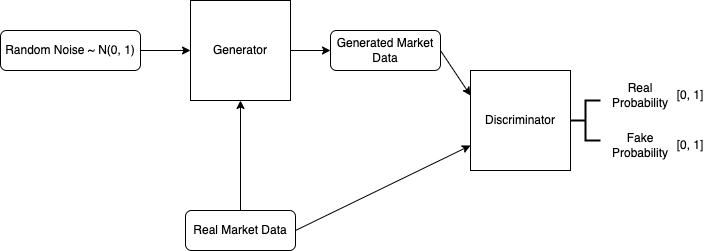
\includegraphics[width=15cm]{templates/assets/gan/gan_architecture.png}
\caption{Structure of a Vanilla GAN}
\end{figure}
\noindent The generator and discriminator compete in a zero-sum game with the objective of training the generator to outperform the discriminator. At each training iteration, the loss is computed given the discriminator's performance and the errors are backpropagated through the generator and discriminator to adjust weights. As the discriminator becomes better at distinguishing real and fake data, the generator has a higher loss and is forced to adjust its weights to generate data that follow the distribution of real data more closely. At the end of the training process, the generator is able to produce new data that resembles the original data, since it has learned the distribution of the real data during the training process.

\subsubsection{Applications of GANs}
GANs have mostly been used for image processing tasks such as generating fake images or performing adversarial attacks on neural networks. However, the framework of GANs can be extended to work with other types of data as well, including tabular and time-series data. This has great implications for working with financial data, as the majority of data in finance consists of tabular and time-series data, such as asset price movement and limit order books. Similar to the GANs used in Deepfake technology, GANs also have the potential to learn the underlying distributions and data-generating processes of price evolution and order books. This allows GANs to learn the market microstructure and price evolution process directly from data instead of relying on various parametric assumptions about market dynamics.

\subsection{Wasserstein GAN (WGAN)}
Nevertheless, vanilla GANs often suffer from a common problem known as mode collapse, where the model hits a local minimum during the training process and is unable to continue learning from the data. Very often, this issue arises with the structure of the GAN due to the non-convexity of the discriminator's loss function during training. Mode collapse ultimately results in the generator producing the same data with the discriminator unable to learn to distinguish this fake. For example, if the generator learns to produce one possible path of simulated market data that is indistinguishable from real market data to the discriminator, then the generator will continue producing this single instance of market data. This can be caused by a variety of factors, with vanishing gradients in the discriminator as one possibility. In order to implement a useful market simulator, the generator component of the GAN must be versatile and learn to generate a large variety of synthetic data that is representative of empirical data. To achieve this versatility, it is essential that the discriminator can perform well during the training process to force the generator to learn to generate a diverse set of useful representations of market data.
\\
\\
Many alternative forms of GANs have been proposed to tackle this issue. One method to address the issue of mode collapse in vanilla GANs is to adjust the output of the discriminator so that it returns a score instead of a probability. Rather than being strictly a classifier of real and fake images, it is possible to turn the discriminator into a critic of generated data instead. This creates the benefit of allowing the discriminator output to exceed the bound of 0 to 1, which can alleviate the effects of vanishing gradients and mode collapse. Arjovsky, Chintala, and Bottou (2017) explore the use of Wasserstein GANs (WGAN) \cite{wgan} to implement this idea by using the Wasserstein loss metric as the output of the discriminator. We will not delve into the derivation of gradient descent, but instead, focus on the implementation with financial data. With a set of 1-Lipschitz functions $D_f$, the Wasserstein GAN value function is defined by:
\begin{equation}
    \min_{G}\max_{D}V_W(D,G) = E_{x\sim p_{data}(x)}[D_f(x)]+E_{z\sim p_{z}(z)}[D_f(G(z))]
\end{equation}
\noindent Instead of making classifications like the discriminator of a VGAN does, the discriminator of a WGAN computes the Wasserstein distance and uses this loss to update weights. The other components of the model remain relatively similar. The structure of a Wasserstein GAN is displayed in Figure 2-2.
\begin{figure}[H]
\centering
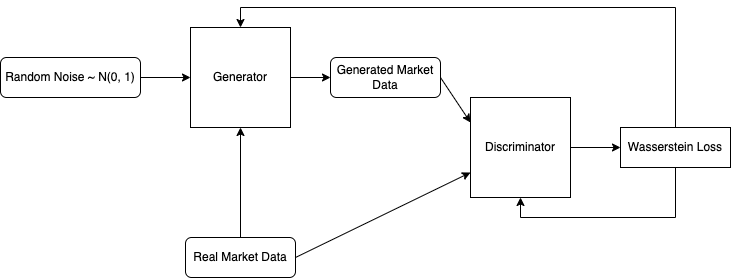
\includegraphics[width=15cm]{templates/assets/gan/wgan_architecture.png}
\caption{Structure of a Wasserstein GAN}
\end{figure}
\noindent For implementing a useful synthetic market environment, the generator must be robust in creating market data from a wide range of possible market conditions and possibilities. Gulrajani et al. (2017) propose an additional improvement to the original WGAN framework by introducing a critic gradient penalty \cite{wgan-gp} instead of the standard weight clipping approach in the training process, which will further help with mitigating mode collapse and promoting stability in data generation. The gradient penalty, combined with the use of Wasserstein distance, greatly improves the GAN's ability to learn robust representations of real market data. This model can now be trained using historical financial data, and the trained generator can be used to construct a representative synthetic market environment which may be useful for a variety of applications, particularly for machine learning methods.

\subsection{Other Forms of GANs}

Additional studies have been done in devising new methods to alter the GAN's structure to improve performance in generating better data. Many other forms of GANs have recently been developed, many of which serve a specific task in data generation. For example, many GANs have been tailored to work particularly on time-series data, which exhibit properties that differ from image data. As time-series data often has high complexities, some variations of GANs are implemented using convolutional and recurrent neural networks in the generators and discriminators to learn sequential data. Olof Mogren (2016) describes Continuous Recurrent Neural Network GANs (C-RNN-GAN) \cite{crnngan}, a variation of GANs, to generate continuous sequential data. Nevertheless, the proposed framework, unlike WGANs, relies on the classification framework and may suffer from mode collapse issues when applied to financial data.

\subsubsection{Time-Series GANs}
One specific feature of time-series data that differs from other types of data is that time-series exhibit various temporal dynamics, which should be preserved when using a GAN to generate time-series data. However, the original framework of GANs does not provide any specific means of learning and maintaining temporal correlations on time series. A notable extension of the GAN framework to work with time-series data is the Time-Series GAN. Jinsung Yoon, Daniel Jarrett, and Mihaela van der Schaar (2019) discuss solutions to this problem and propose a modification of GANs to generate more-realistic time-series data that maintain statistical and temporal properties \cite{tsgan}. The Time-Series GAN (TimeGAN) preserves the temporal dynamics of time-series data by introducing a step-wise supervised loss to allow the generator and discriminator to learn the conditional distribution of the data, as well as an embedding network to reduce the dimensionality of the feature space during training. TimeGAN combines the adversarial learning framework with autoencoders to simultaneously learn and optimize the supervised and unsupervised losses, as shown below.
\begin{figure}[H]
\centering
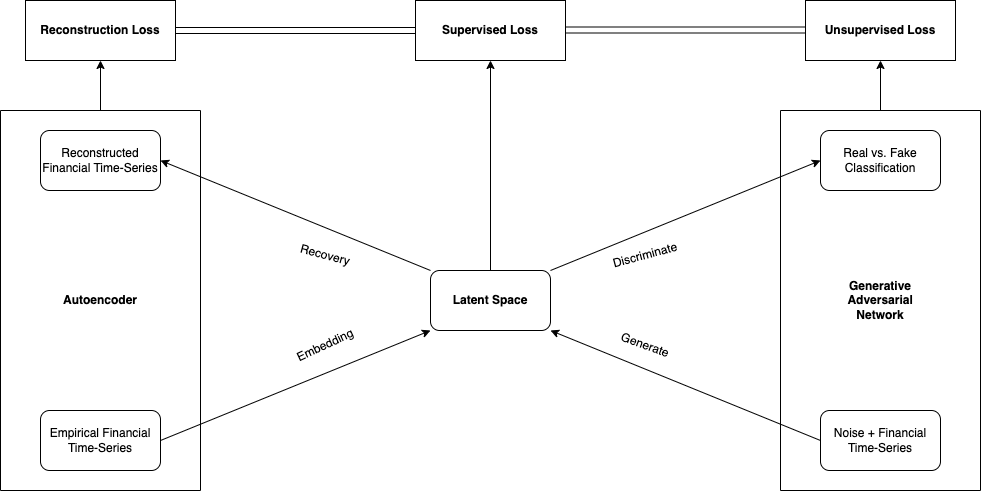
\includegraphics[width=15cm]{templates/assets/gan/tsgan_architecture.png}
\caption{Structure of a Time-Series GAN}
\end{figure}

\section{Using GANs for Synthetic Data Generation}
Although state-of-the-art applications of GANs involve image processing tasks, this framework can be adapted to work with data other than images, including tabular and time-series data. The goal of using GANs as an alternative approach to generating and simulating data is to remove the need for parameterization and assumptions about market dynamics. Since GANs are an unsupervised learning and non-parametric framework, they learn the distribution directly from real data instead of relying on the careful selection of parameters.
\\
\\
The trained generator portion of the GAN can be used to generate new data given a starting point and random noise input. During the synthetic data generation process, the discriminator portion of the GAN is not required, as it served its primary purpose of improving the generator and helping it learn the underlying data-generating process during training. As discussed before, the objective of the GAN is to generate a diverse set of possible market scenarios representative of the true patterns and dynamics observed in empirical market data. In the context of simulating financial time-series data of spot prices in the market, this translates into using the generator to generate spot price paths that have relatively similar distributional statistics and movement patterns to real spot price data.
\\
\\
Markets can be bullish, bearish, or stagnant at most points in time, but true market dynamics can be incredibly complex and noisy which presents a huge challenge for working with financial data. Ideally, the generator will be able to simulate many possible market scenarios that are representative of the complexity and noisiness present in empirical data. The possibilities and randomness of market dynamics are represented as random noise inputted into the generator when generating data.
\subsection{Simulating Financial Market Data with GANs}
Although the model can be adapted to work with any asset that has historical data available, we will focus on using the trained model for a specific stock, such as Apple (AAPL). AAPL has an abundance of historical price data available, dating back to the 1980s, with over 40 years of data. The generator requires a starting point in the financial time series to then input random noise and generate new data. Of course, at any point in time during the life of the company, there is a current price level and an unpredictable and uncertain future trend. Being able to simulate many realistically possible paths of data can be useful for training and evaluating algorithms that require an abundance of data. With the trained GAN, a large number of data points can be generated by simply producing random noise as input. The generator uses a starting point and combines random noise with the underlying distribution it has learned during training. Using the trained generator to simulate one path of spot prices for AAPL yields the following results displayed below.
\begin{figure}[h]
\centering
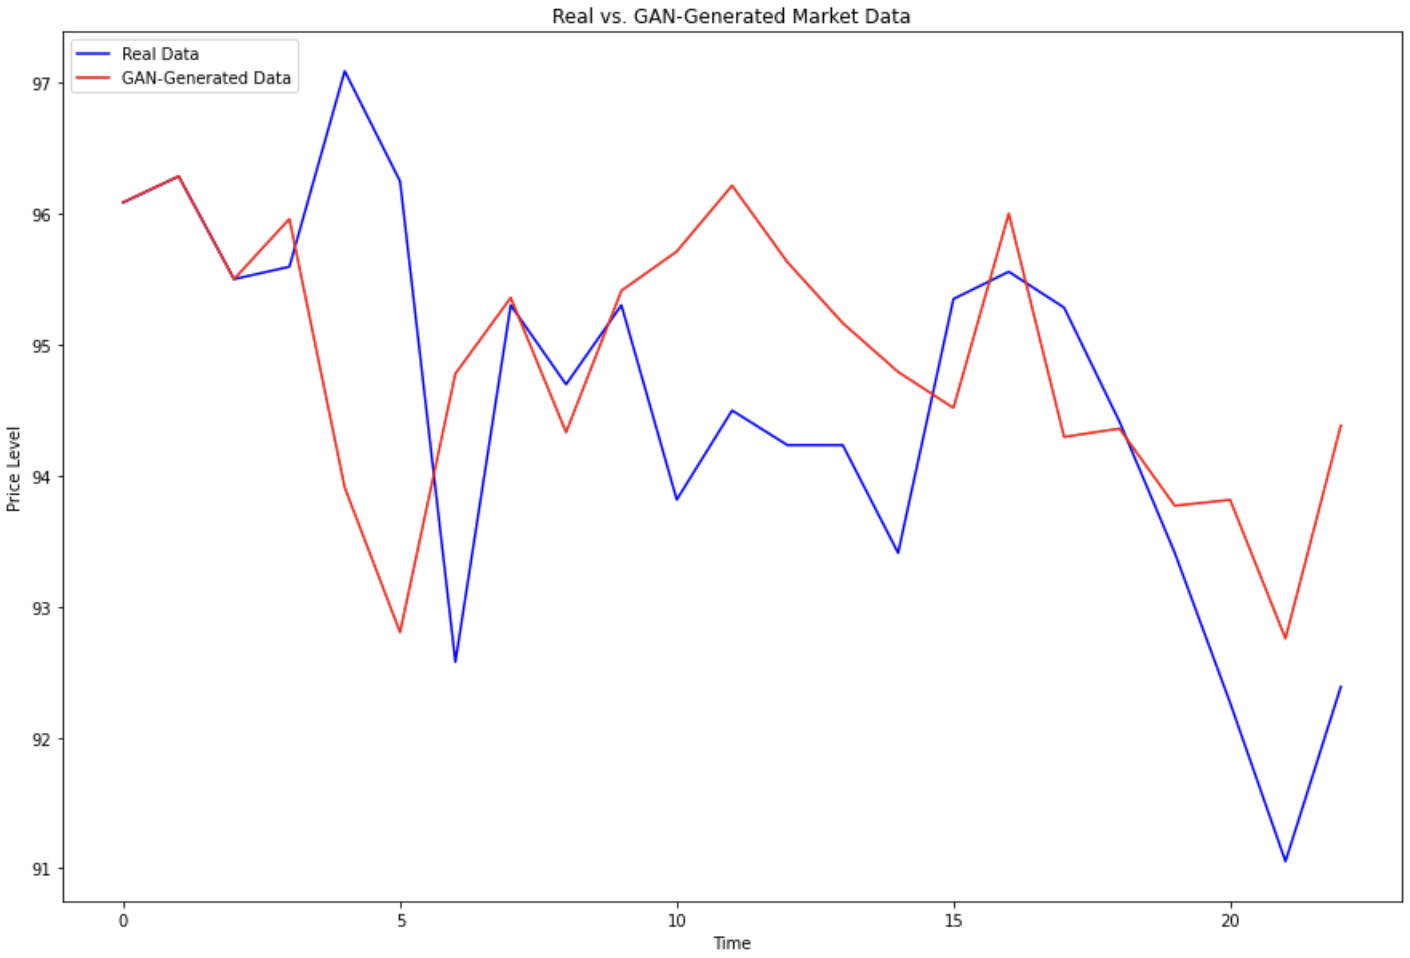
\includegraphics[width=14.5cm]{templates/assets/gan/gan_stable.png}
\caption{GAN-Based Spot Price Simulation}
\end{figure}
\\
\noindent As we can qualitatively see in the plot above, the generated data exhibits similar properties as the real data and has similar movement patterns. The real and generated data both have the same starting point, at a price level of around \$96, but the GAN has learned the dynamics of AAPL's historic price movement and has generated another plausible scenario of how the price might have evolved over time. This systematic data generation framework has great implications for a variety of financial applications, most importantly enhancing algorithms that require lots of data. The generation of many alternative paths from a starting point can be used as data to train and evaluate models and strategies. Ideally, the models and strategies that traders and investors develop are robust to different market conditions and possibilities, which can be captured by the AI-generated data trained on historical data.
\\ \\
For example, the generator of the GAN would ideally be able to produce a diverse set of market data, including data under both bullish and bearish markets. Using the trained generator, the diagrams below show AI-generated instances of the evolution of AAPL in bullish and bearish conditions.
\begin{figure}[h]
\centering
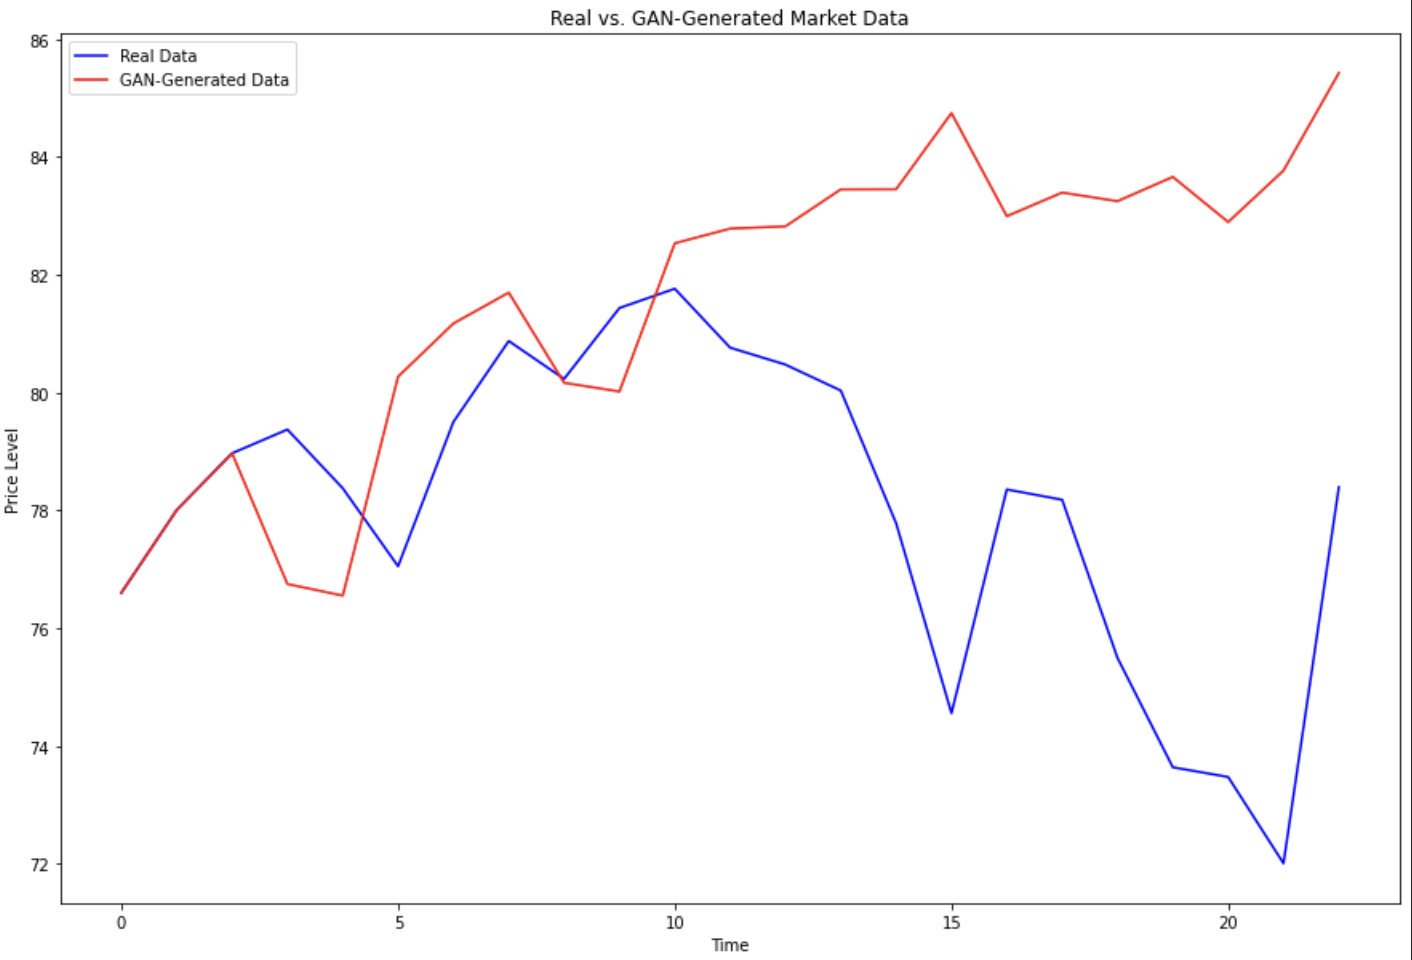
\includegraphics[width=11cm]{templates/assets/gan/gan_up.png}
\caption{Upwards Trend Path Simulated by GAN}
\end{figure}
\begin{figure}[h]
\centering
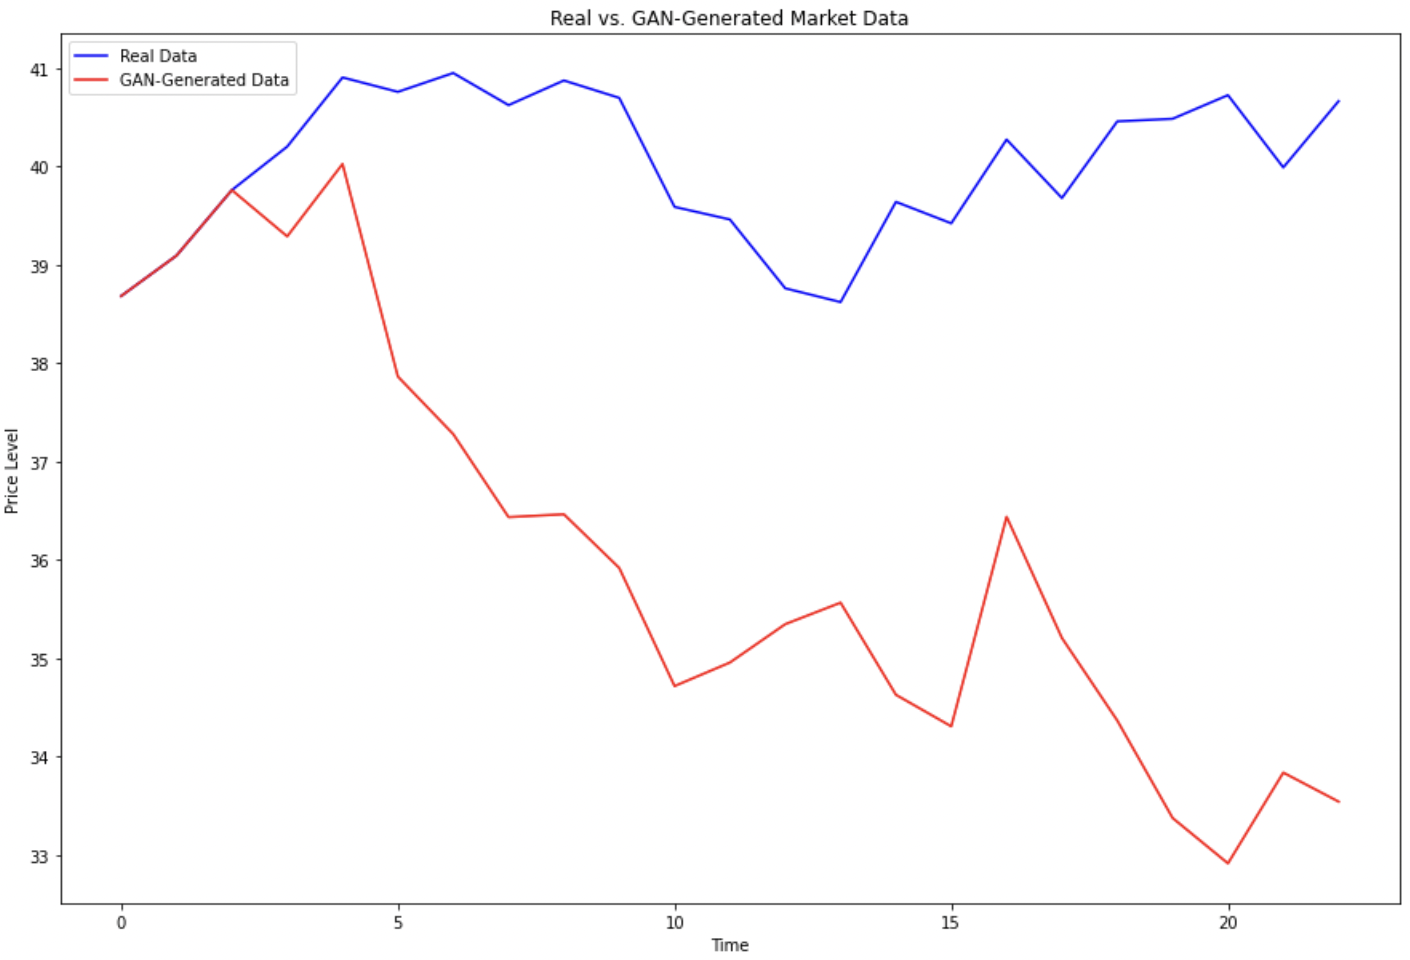
\includegraphics[width=11cm]{templates/assets/gan/gan_down.png}
\caption{Downwards Trend Path Simulated by GAN}
\end{figure}
\\
\noindent The figure above shows an AI-generated path that has an upward trend compared to the real historical data. As shown above, the red lines represents the GAN-generated data and the blue lines represents the actual data. In figure 2-5, the generated data appears to have an upward trend relative to the actual historical data, while in figure 2-6, the generated data appears to have a downward trend relative to the actual historical data. Although the real and generated data have different trends, the temporal properties of stock price dynamics appear to be relatively similar. This divergence in the real and generated paths, along with the preservation of price movement dynamics, is essential for being able to use GAN-generated data for training and evaluating models and strategies. It is possible to use this generator to generate an abundance of realistic market data under various market scenarios, similar to using Monte Carlo simulations. The difference is that while Monte Carlo simulations are parametric and probability-based, which may not capture the complexities and patterns of real market dynamics, GAN-generated data exhibits properties similar to empirical data and has a similar underlying distribution. It is interesting to observe, however, that a plot of GAN-generated series looks very similar to Monte Carlo simulations since both methods capture a variety of possibilities of stock price movement. A plot of GAN-based market simulation for AAPL is displayed below.
\begin{figure}[h]
\centering
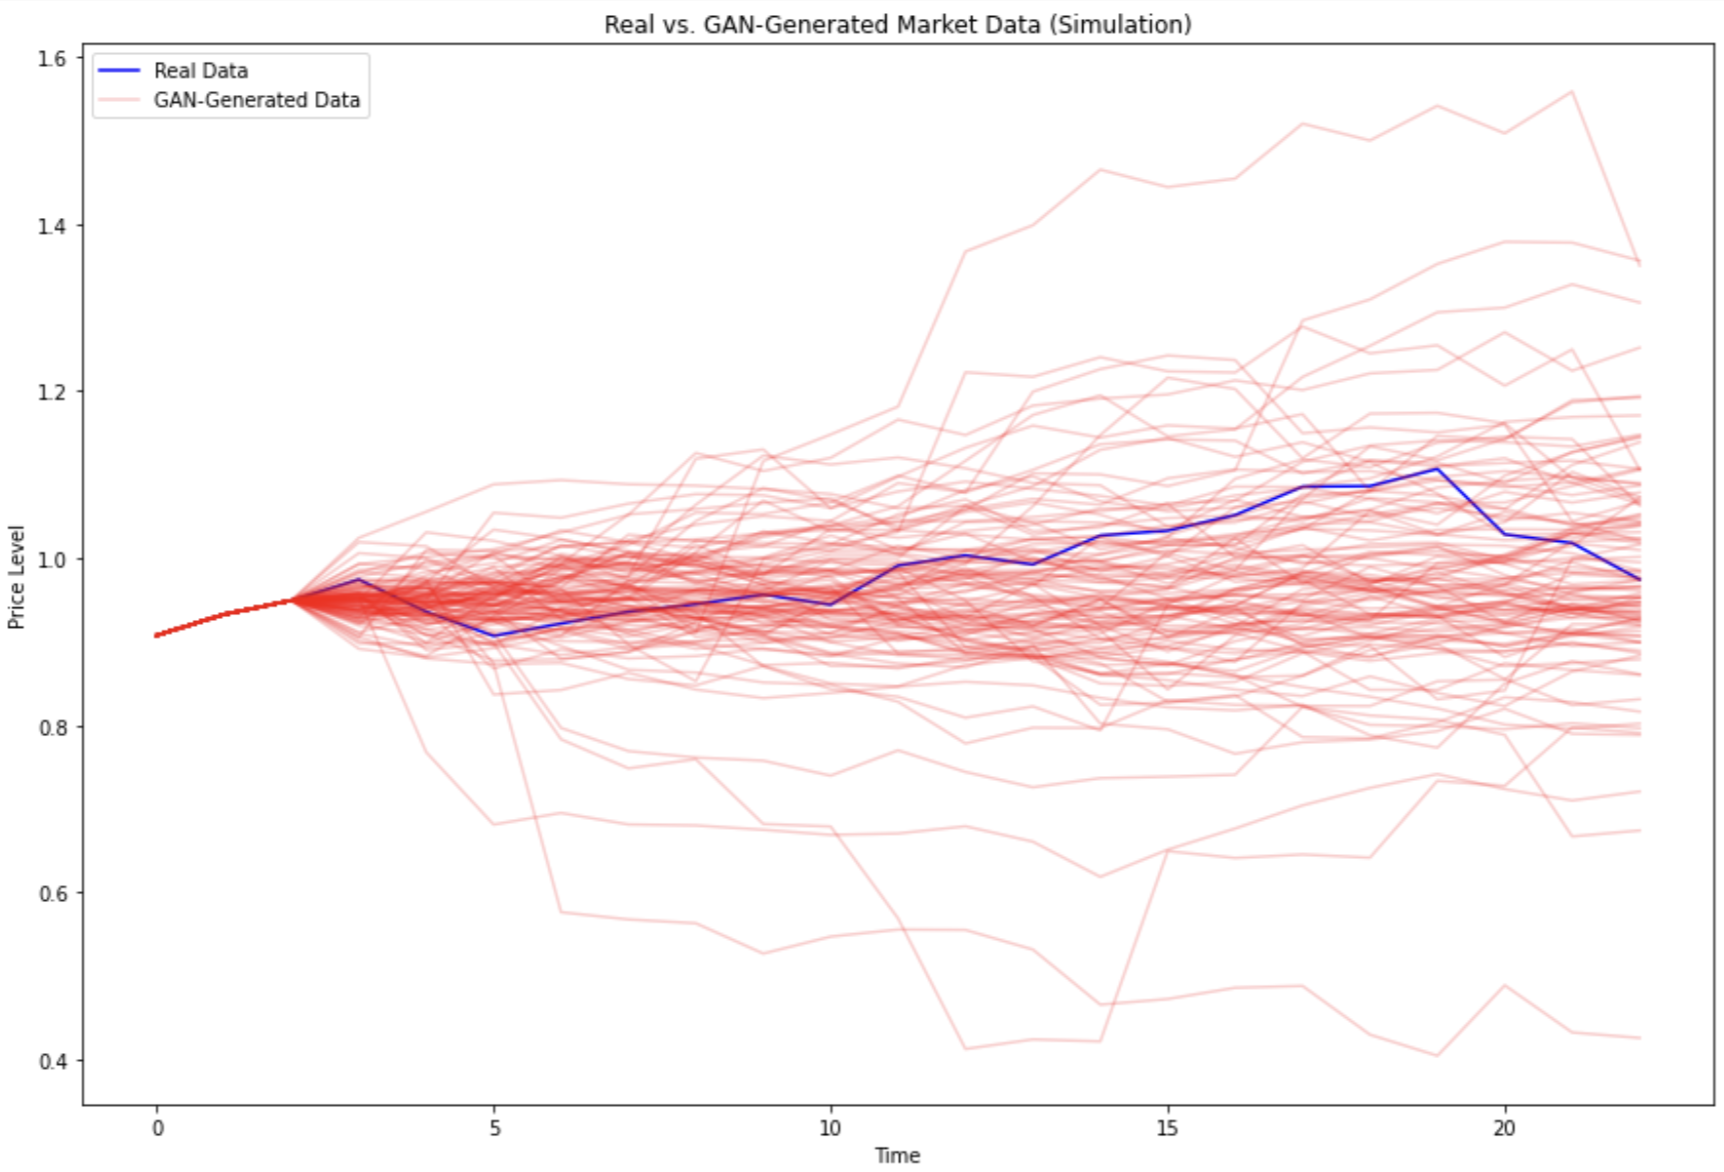
\includegraphics[width=14cm]{templates/assets/gan/gan_simulation.png}
\caption{GAN-Based Market Simulation of Price Paths}
\end{figure}

\section{Evaluating GAN-Based Market Simulations}
To be confident in the accuracy of GAN-generated market data in representing empirical data, there must be a systematic framework for quantitatively evaluating the similarity of synthetic data to real data. Unlike synthetic image generation with GANs, where the quality of the generated data can be visually observed by humans, synthetic time series and financial data are harder to evaluate directly. It is easier for humans to observe the facial features of generated images than it is to identify common-occurring statistical properties present in time series data.
\\
\\
However, since GANs are an unsupervised machine learning framework, there isn't a single or standard way to evaluate performance. With supervised machine learning methods, the standard way of measuring performance is to make predictions on a test data set and compute a metric such as accuracy or root mean square error. Since GANs are generating new data, it is infeasible to use the same evaluation methods. However, this does not mean that the similarity between GAN-generated synthetic data and real data cannot be measured. In fact, there are various metrics and statistics apparent in time-series data that can be measured, evaluated, and compared between synthetic market data and real market data. Ideally, these metrics will be similar in value which indicates that the GAN has learned the underlying distribution of the financial time-series data. Although it is difficult to explain GAN outputs, the metrics will bring confidence into the GAN learning market dynamics from data.

\subsection{Time-Series Distributional Statistics \& Metrics}

There are various time-series metrics and statistics that can be computed that describe the temporal dynamics and conditional distribution of the time-series data. For example, distributional statistics such as mean, median, minimum, and maximum may be useful for comparing real and synthetic data to ensure the synthetic data has a relatively similar distribution. There should be some degree of variation in the statistics so that the GAN is able to generate a diverse set of data.
\\
However, properties that exist in financial time-series data are often more complex in nature. It is simple to generate data with similar distributional statistics, as Monte Carlo methods do well, but difficult to mimic the exact temporal features that exist in financial data, since the exact properties of stock returns are unknown. To quantitatively evaluate the ability of the GAN to generate meaningful representations of market data, time-series feature extraction can be used. Maximilian Christ et al. (2018) explore various time-series feature extraction \cite{tsfresh} methods to gain insight into the temporal dynamics of time-series data. The \textbf{tsfresh} package encapsulates over 794 time-series features that can be used to describe the properties and behaviors of time-series data. A comprehensive list of all extracted features can be found on the official \textbf{tsfresh} documentation page. Taking the GAN-generated data and real market data, a summary of the time-series metrics is displayed below.
\begin{table}[h]
\begin{centering}
\begin{tabular}{@{\extracolsep{2pt}}lcccccc}
\toprule
                        & Mean   & Median   & Variance & Skewness & Kurtosis \\ \midrule
Real Market Data &   0.76          &   0.77       &     0.77      &      0.80        &           &           \\
GAN Market Data        &     0.48        &    0.48      &     0.47      &       0.57       &           &           \\ \bottomrule
\end{tabular}
\caption{Distributional Statistics of Real vs. GAN-Generated Market Data}
\end{centering}
\end{table}

\begin{table}[h]
\begin{centering}
\begin{tabular}{@{\extracolsep{2pt}}lcccccc}
\toprule
                        & Mean   & Median   & Variance & Skewness & Kurtosis \\ \midrule
Real Market Data &   0.76          &   0.77       &     0.77      &      0.80        &           &           \\
GAN Market Data        &     0.48        &    0.48      &     0.47      &       0.57       &           &           \\ \bottomrule
\end{tabular}
\caption{Autocorrelation of Real vs. GAN-Generated Market Data}
\end{centering}
\end{table}

\noindent As can be seen from the distributional statistics and autocorrelations of the real and GAN-generated market data above, they appear to have similar properties.

\subsection{t-SNE Comparison}
There are a large number of time-series features to compare manually. One method to evaluate how similar the metrics of the generator's synthetic data are to the empirical data is to use the t-SNE \cite{tsne} algorithm. As high-dimensional data is very difficult to visualize, the t-distributed stochastic neighbor embedding (t-SNE) method visualizes the high-dimensional inputs by mapping the data from a high-dimension to a low-dimension. Using this method, we can compare the t-SNE mapping visualizations between the time-series metrics of generated market data and real market data. Using the generator to generate 1000 samples, the t-SNE plot of real (teal) and synthetic (red) financial time-series data metrics is displayed below.
\begin{figure}[h]
\centering
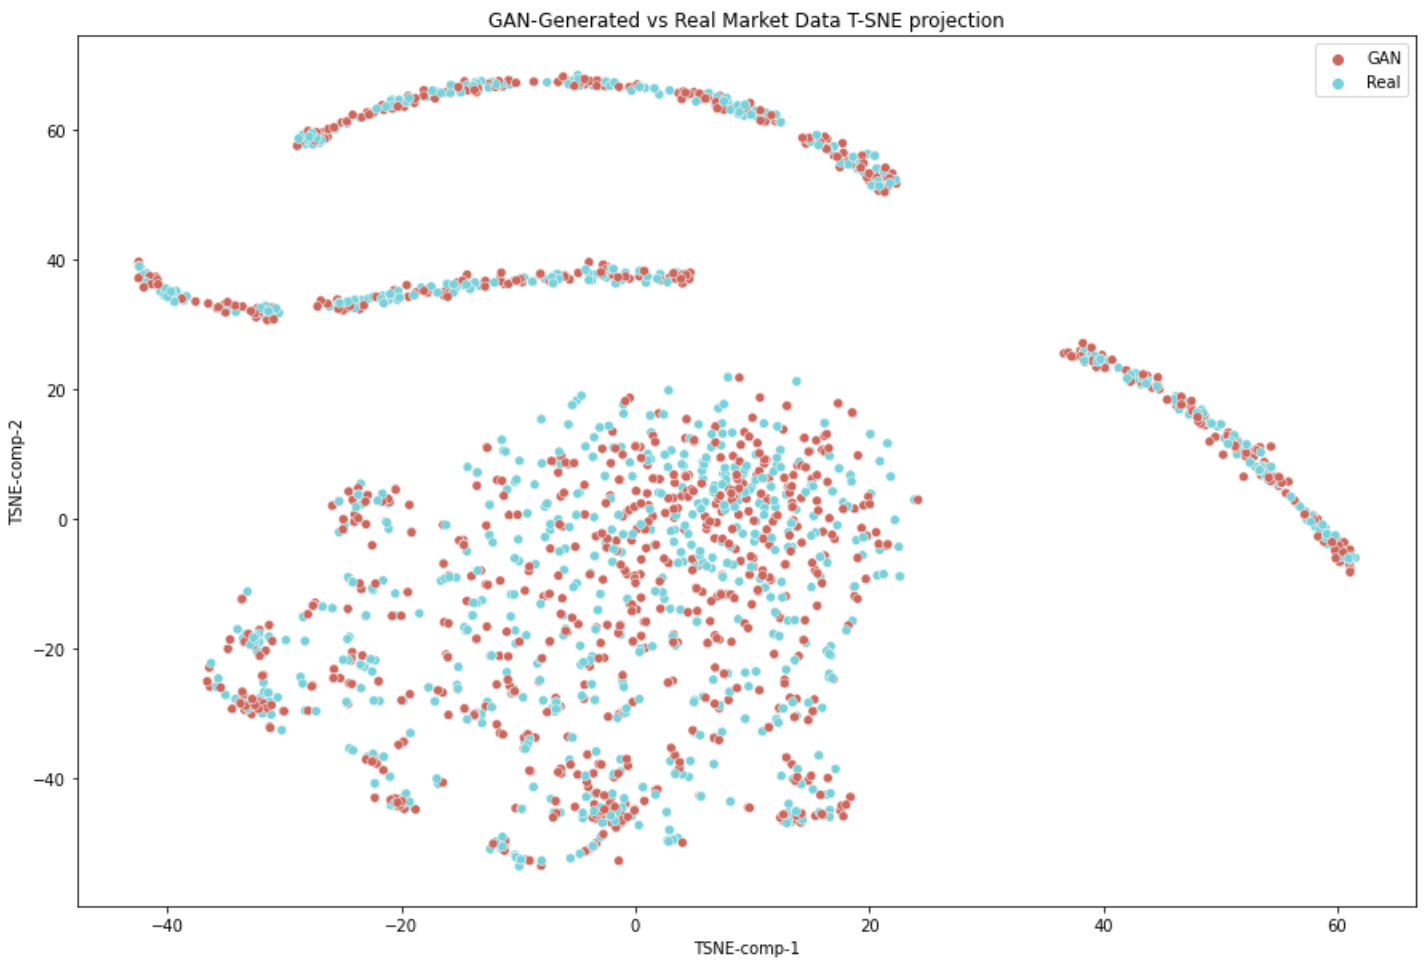
\includegraphics[width=14cm]{templates/assets/gan/tsne.png}
\caption{t-SNE Visualization of Real vs. Synthetic Market Data}
\end{figure}
\\
The t-SNE visualization shows that the high-to-low dimensional mapping of the real data closely follows that of the GAN-generated data. This shows that the statistics and time-series features previously described are similar for both real and synthetic data, implying the GAN's ability to learn the properties of empirical stock returns.

\appendix
\chapter{Tables}

\begin{table}
\caption{Armadillos}
\label{arm:table}
\begin{center}
\begin{tabular}{||l|l||}\hline
Armadillos & are \\\hline
our	   & friends \\\hline
\end{tabular}
\end{center}
\end{table}

\clearpage
\newpage

\chapter{Figures}

\vspace*{-3in}

\begin{figure}
\vspace{2.4in}
\caption{Armadillo slaying lawyer.}
\label{arm:fig1}
\end{figure}
\clearpage
\newpage

\begin{figure}
\vspace{2.4in}
\caption{Armadillo eradicating national debt.}
\label{arm:fig2}
\end{figure}
\clearpage
\newpage

%% This defines the bibliography file (main.bib) and the bibliography style.
%% If you want to create a bibliography file by hand, change the contents of
%% this file to a `thebibliography' environment.  For more information 
%% see section 4.3 of the LaTeX manual.
\begin{singlespace}
\bibliography{main}
\bibliographystyle{plain}
\end{singlespace}

\end{document}

